\documentclass[times, utf8, zavrsni, numeric]{fer}
\usepackage{booktabs}
\usepackage{url}
\usepackage{listing}
\usepackage[hidelinks]{hyperref}

\begin{document}

% TODO: Navedite broj rada.
\thesisnumber{5173}

\title{Implementacija jezgre RTS igre}

\author{Leon Luttenberger}

\maketitle

% Ispis stranice s napomenom o umetanju izvornika rada. Uklonite naredbu \izvornik ako želite izbaciti tu stranicu.
\izvornik{}

% Dodavanje zahvale ili prazne stranice. Ako ne želite dodati zahvalu, naredbu ostavite radi prazne stranice.
\zahvala{}

\tableofcontents

\chapter{Uvod}
% \par Strategije u stvarnom vremenu (engl. \textit{Real-Time Strategy}, u nastavku RTS) su žanr računalnih igara temeljene na skupljanju resursa za izgradnju jedinica i građevina s ciljem da se poraze protivnici. Za razliku od strategija na potez (engl. Turn-based strategy) gdje svaki igrač ima proizvoljno vrijeme za odigrati svoj potez, u RTS igrama svi igrači igraju svoje poteze u isto vrijeme znajući da svi protivnici rade isto. U širom smislu, RTS igra se može definirati kao simulacija bitke u stvarnom vremenu\cite{url:WhatDoesRTSMean}.

% \par Odluke u RTS igrama se svode na dvije kategorije: mikro upravljanje i marko upravljanje\cite{article:HybridPathdinding}. Makro upravljanje predstavlja odluke na višoj razini apstrakcije, npr. koje jedinice i koje građevine graditi, kada započeti napad na protivnika, koje nadogradnje kupovati, itd. Mikro upravljanje se svodi na upravljanje samih jedinica, poput taktičkog pozicioniranja jedinica i uporabe njihovih specijalnih mogućnosti.

% \par Još jedna zanimljivost kod RTS igara se sastoji od mnogih podsustava koji nisu specifični za konkretnu igru, te ih je moguće izolirate u zasebne komponente:
% \begin{itemize}
%     \item prikaz mape.
%     \item kretanje jedinica po mapi.
%     \item sustav upravljanja resursima.
% \end{itemize}

% \par Kretanje jedinica po mapi u okruženjima koji su nepoznati ili čije se stanje može promijeniti u stvarnom vremenu predstavlja poseban izazov. Naime, kretanje jedinica prema zadanom cilju mora glatko te moraju izvoditi pretragu u stvarnom vremenu. Nadalje, ako je cilj zadan nad grupom jedinicama, očekivano je da će se odabrane jedinice grupirati i kretati zajedno prema cilju. Moguća rješenja za ove probleme bit će obrađena u poglavlju \ref{pathfinding}.

\chapter{Pregled vrsti računalnih igara}\label{ch:games}

\chapter{RTS igre}\label{ch:rtsGames}
RTS žanr računalnih igara temelje se na skupljanju resursa za izgradnju jedinica i građevina s ciljem da se poraze protivnici. 
Za razliku od ranije navedenih strategija na potez (engl. Turn-based strategy) gdje svaki igrač ima proizvoljno vrijeme za odigrati svoj potez, u RTS igrama svi igrači igraju svoje poteze u isto vrijeme znajući da svi protivnici rade isto. 
U širem smislu, RTS igra se može definirati kao simulacija bitke u stvarnom vremenu\cite{url:WhatDoesRTSMean}.

%TODO napisi o cemu ce sve bit poglavlje

\section{Elementi RTS žanra}

\par Tipična RTS igra sastoji se od mnogih različitih elemenata.
Prije svega, svaka igra se odvija na mapi ograničene veličine koja je određena s raznim tipovima terena, poput trave, vode, planina, pustinje, itd. 
Tip terena može odrediti koje se jedinice mogu kretati po njemu.
Primjerice, pravila igre mogu biti takva da se običan vojnik ne može kretati po vodi, dok neki drugi tip jedinice poput broda može.
Kao posljedica toga, teren igra veliku ulogu jer može zahtijevati korištenje posebnih strategija.

\par Još jedna bitan element RTS igara je skupljanje resursa.
Ovisno o konkretnoj igri, resursi mogu biti drvo, minerali, nafta, zlato, itd. Oni se tipično skupljaju s posebnom vrstom jedinica zvanom radnicima, te se koriste za izgradnju novih jedinica, zgrada, radnika, itd.
Resursi također igraju veliku ulogu u strategiji same igre.
Primjerice, ako se igrač nalazi u situaciji gdje ne može dalje napredovati zbog manjka nekog resursa, bit će prisiljen otići u potragu za istim.
Analogno tome, višak izvora nekog resursa igrača može postaviti u opasnost jer će ostalim sudionicima igre biti prioritet napasti s ciljem da se ukradu resursi.

\par Osim resursa i mape, bitan element u svakoj RTS igri je izgradnja zgrada. 
Konkretne igre obično imaju mnogo različitih zgrada od kojih svaka ima svoj skup funkcionalnosti, poput treniranja novih jedinica, procesiranje resursa, istraživanje novih tehnologija, itd.  

\par Posljednji bitni element igara u RTS žanru su jedinice. 
Svaka igra ima skup različitih jedinica koje igrač može odabrati i izgraditi za svoju vojsku.
Svaka vrsta jedinice može imati svoje prednosti i mane.
Npr.\ igra može kao vrstu jedinice imati konjanika koja ima prednost brzog kretanja po mapi, no ima manu da je izrazito ranjiv na kopljanike.

\par Bitno je naglasiti da dosad navedeni elementi nisu direktno ovisni jedni o drugima.
Mapa može biti definirana izvan same igre u nekom vanjskom uređivaču mapa, dok jedinice, resursi i zgrade ne moraju ništa konkretno znati jedni o drugima.
Jedinice će samo znati da se kreću po terenu čiji koji ima neke definirane karakteristike, te će samo znati da napada protivničke zgrade i jedinice. 
Zgrade i resursi mogu biti definirani samo kao objekti na mapi, gdje će bilo kakva daljnja funkcionalnost ovisiti o konkretnoj igri.
% TODO dodaj referencu na poglavlje o implementacij

\section{Strategija}

\par Glavni cilj u igrama u RTS žanru analogan je igrama poput šaha, odnosno cilj je pametnom uporabom vlastite vojske poraziti vojsku od suparnika. 
Za razliku od šaha, u računalnim strateškim igrama igrač započne igru \textit{praznih ruku}, odnosno igru može započeti sa samo jednim radnikom čiji je posao skupiti prve resurse s kojima će izgraditi prve jedinice te nove radnike i zgrade.

\par Igrač jedinicama daje naredbe tako da ih odabere (npr.\ pritiskom tipke miša) i zada im odredište gdje se moraju pomaknut ili protivničku jedinicu koju moraju napasti. 
Igrač također može odabrati zgradu i njoj dati naredbu što da proizvodi, poput novih jedinica ili istraživanja novih tehnologija koje će omogućiti izgradnju novih tipova jedinica i zgrada.

\par Odluke u RTS igrama mogu se podijeliti u dvije kategorije: mikro upravljanje i makro upravljanje. 
Makro upravljanje predstavlja odluke na višoj razini apstrakcije poput odluka koje zgrade i jedinice graditi, kada krenuti u napad, itd. 
Mikro upravljanje svodi se na upravljanje pojedinim jedinicama.
Dobro taktičko pozicioniranje jedinica i fokus na najjače protivničke jedinice u dosegu često mogu definirati ishod igre.\cite{article:HybridPathdinding}

\par Kao posljedica svega navedenog, evidentno je da je strategija centralnih aspekt igara u RTS žanru. 

\par Također, bitno je naglasiti da će određene strategije funkcionirati samo protiv pojedinih protivnika i da određene situacije mogu zahtijevati promjenu strategije. 
Primjerice, igrač se može odlučiti za strategiju ranog napada (engl. \textit{rush strategy}), odnosno odmah se fokusirati na izgradnju velikog broja osnovnih borbenih jedinica koje će što ranije moguće poslati u napad na protivnika.
Kao kontrast tome, protivnik se može fokusirati na razvoj tehnologije što će ga ostaviti ranjivim na početku igre, ali će mu u kasnijim fazama igre omogućiti da gradi jedinice koje su jače od protivničkih.

\section{Izazov za umjetnu inteligenciju}

\par RTS igre predstavljaju razne izazove za razvoj umjetne inteligencije. 
Iz perspektive mikro upravljanja, umjetna inteligencija mora imati sustav po kojem će određivati najkraći put do odredišta, te kako se treba ponašati u slučaju da na putu naiđe na nešto ne planirano, poput protivničkih jedinica ili promjena na terenu.

%TODO

\section{Primjeri popularnih RTS igara}

\chapter{Kretanje jedinica}\label{ch:pathfinding}

\section{Pretraživanje prostora stanja}\label{sec:stateSearch}
\par Pretraživanje prostore stanja može riješiti mnogo analitičkih problema, uključujući pronalazak najkraćeg puta. 
Ako korisnik odabere jedinicu koja se nalazi na početnoj poziciji i zada joj odredište, jedinica će pretragom prostornog stanja pronaći slijed akcija koji definira optimalni put.

\par Problem pretrage \(S\) možemo formulirati s petorkom
\[(S, S_0, akcije(s), prijelaz(s, a), cilj(s), cijena(s, a))\]
u kojoj su:
\begin{itemize}
    \item \(S\) skup stanja.
    \item \(S_0\) početno stanje.
    \item \(akcije(s)\) skup mogućih akcija za stanje \(s\).
    \item \(prijelaz(s, a)\) stanje koje nastane kada se izvede akcija \(a\) u stanju \(s\).
    \item \(cilj(s)\) ispituje jeli stanje \(s\) ciljno stanje.
    \item \(cijena(s, a)\) cijena akcije \(a\) kada smo u stanju \(s\). 
\end{itemize}

\subsection{Neusmjerena pretraga}

\begin{figure}[h] 
	\centering
	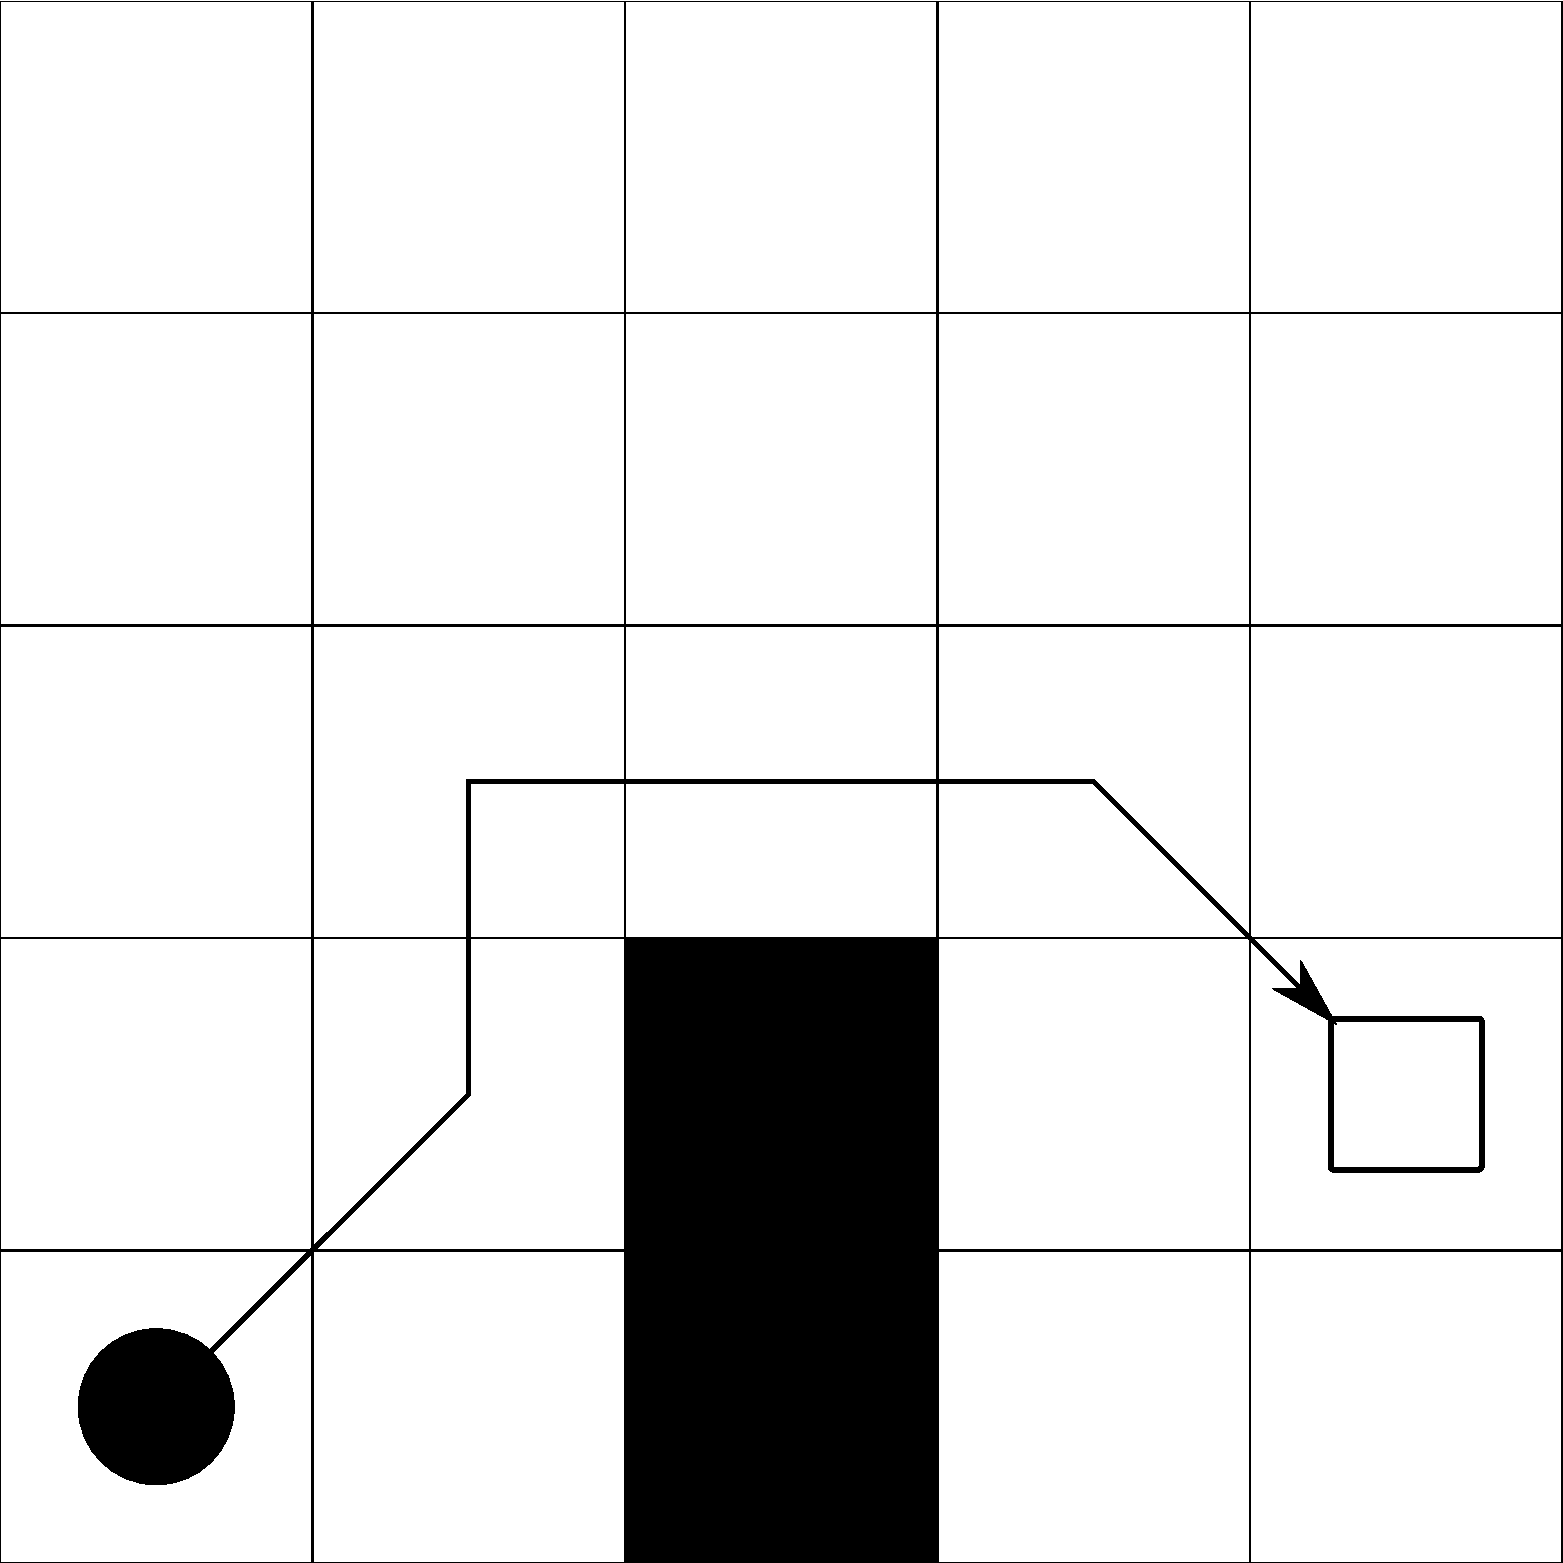
\includegraphics[width=0.3\linewidth]{images/basicGrid.pdf}
	\caption{}
	\label{fig:basicGrid}
\end{figure} 

Na slici~\ref{fig:basicGrid} prikazan je rezultat pretrage najkraćeg puta na 5x5 ploči na kojoj su mogući i dijagonalni prijelazi.
Ispunjeni krug predstavlja početnu poziciju, prazan kvadrat predstavlja cilj te ispunjeni kvadrati predstavljaju prepreke.
Ako definirano da se pločica u donjem lijevog predstavlja s koordinatama \((0, 0)\), tada standardna formulacija problema glasi:
\begin{itemize}
    \item \(S\): sve pozicije od \((0, 0)\) i \((4, 4)\).
    \item \(S_0\): stanje \((0, 0)\).
    \item \(akcije(s)\): predstavlja prijelaze s kojima se može doći do susjednih polja od \(s\) koji nisu prepreke. 
    Moguće vrijednosti su: \textit{gore}, \textit{dolje}, \textit{lijevo}, \textit{desno}, \textit{gore-lijevo}, \textit{dolje-lijevo}, \textit{gore-desno} i \textit{dolje-desno}. 
    Npr.\ za početno stanje \(S_0\) funkcija će vrati slijed: \textit{gore}, \textit{desno} i \textit{gore-desno}. 
    \item \(prijelaz(s, a)\): funkcija vraća novu poziciju na polju kada se akcija \(a\) izvrši iz stanja \(s\). Npr. \(prijelaz((0, 1), gore)\) će vratiti stanje \((1, 1)\).
    \item \(cilj(s)\): funkcija je zadovoljena samo za \((4, 1)\).
    \item \(cijena(s, a)\): cijene prijelaza su Euklidove udaljenosti, odnosno prijelazi na strogo susjedna polja imaju cijenu \(1\), dok dijagonalni prijelazi imaju trošak \(\sqrt{2}\).
\end{itemize}

\par S obzirom na činjenicu da cijene prijelaza nisu uvijek iste, potrebno je odabrati algoritam pretrage koji uzima u obzir cijenu puta.
Najosnovniji takav algoritam pretrage je \textbf{pretraživanje s jednolikom cijenom} (engl. \textit{uniform-cost search}). 
Algoritam koristi prioritetni red u kojeg stavlja čvorove s njihovom ukupnom udaljenosti od početnog stanja \(g(s)\), što osigurava da će svako stanje biti posjećeno s najkraćim mogućim putem.
Zbog navedenog svojstva, vidi se da je algoritam \textbf{optimalan}, odnosno uvijek će pronaći optimalni put do odredišta ako ono postoji.
%TODO dodati pseudokod

\par Unatoč tome što će algoritam uvijek pronaći najkraći put, ponekad će za to morati posjetiti veliki broj stanja jer se u obzir uzima samo cijena puta, bez znanja o tome dali je taj čvor bliži cilju ili ne. 
Zbog ovog svojstva pretraživanje s jednolikom cijenom čini jedno od neusmjerenih algoritama pretrage.

\subsection{Usmjerena pretraga}

\par Usmjereni algoritmi pretraživanja su algoritmi koji koriste heurističku informaciju kako bi se pretraživanje brže usmjerilo prema cilju.
U općenitom obliku ovakvog algoritma stanja se ubacuju u prioritetni red kao u pretraživanju s jednolikom cijenom, no umjesto da se koristi cijena puta \(g(s)\) koristi se \textbf{evaluacijska funkcija} \(f(s)\).

\par Odabir evaluacijske funkcije \(f\) definira strategiju pretrage. 
Funkcija \(f\) tipično ima kao komponentu \textbf{heurističku funkciju} \(h\), koja se definira kao procjena minimalnog troška puta od trenutnog čvora do cilja\cite{book:AIModernApproach}.

\par Primjer takvog pretraživanje je pohlepno pretraživanje. 
Ono odabire onaj čvor koji se čini najbliži cilju, ne uzimajući u obzir trošak puta.
Evaluacijska funkcija \(f(s)\) se definira kao \(f(s) = h(s)\).
% TODO dodati primjer

\par Poboljšanje tog algoritma je ujedno i najpoznatija implementacija usmjerene pretrage: \textbf{algoritam A*}. 
U njemu se čvorovi evaluiraju tako da se zbroji trošak puta \(g(s)\) i heuristika \(h(s)\): 
\[f(s) = g(s) + h(s).\]
Prema tome, vrijednost \(f(s)\) predstavlja procjenu troška puta koji prolazi kroz stanje \(s\).
Ovaj algoritam je identičan pretraživanju s jednolikom cijenom, osim što se u prioritetni red za čvorove ubacuje vrijednost \(g(s) + h(s)\) umjesto \(g(s)\).

\subsubsection{Uvjeti za optimalnost algoritma A*}
Kako bi algoritam A* bio optimalan, heuristika mora zadovoljiti sljedeća dva svojstva: \textbf{optimističnost} i \textbf{konzistentnost}.

\par Heuristika je optimistična ako nikad ne predvidi udaljenost do cilja koja je veća od stvarne. 
Kao posljedica činjenice da je \(g(s)\) cijena puta do stanja \(s\), \(f(s)\) nikad neće imati vrijednost veću od cijene stvarnog puta do cilja kroz čvor \(s\).
Matematički formulirano, ako je \(h^*(s)\) cijena stvarnog puta od čvora \(s\) do cilja, tada vrijedi:
\[\forall s \in S, h(s) \leq h^*(s).\]
Također, vrijednost heuristike u ciljnom čvoru mora biti 0: \(h(s_{cilj}) = 0\).

\par Heuristika je konzistentna ako je procjena udaljenosti do cilja manja ili jednaka zbroju udaljenosti do cilja od susjednog stanja i cijeni puta između navedena dva stanja.
Odnosno, ako je \(s\) trenutno stanje, \(s'\) susjedno stanje i \(a\) akcija koja vodi iz \(s\) u \(s'\), tada vrijedi:
\[h(s) \leq c(s, a) + h(s').\]

\par Konzistentna heuristika je ujedno i optimistična, iako suprotno ne vrijedi. 
Samim time, konzistentnost je stroži uvjet od optimističnosti. 
U algoritmu A* konzistentnost heuristike osigurava da će se čvor proširiti kada je najkraći put do njega pronađen, poput pretraživanja s jednolikom cijenom.

% TODO napiši nešto to obaviještenosti heuristike

% TODO dodaj koji primjer

\section{Prilagodba na promjene}\label{sec:adaptation}

\par Likovi u računalnim igrama se moraju kretati glatko bez nepotrebnih stajanja, što znači da moraju pretraživati u realnom vremenu. 
A* sam po sebi nije prikladan za taj posao, jer broj stanja koji se moraju pretražiti raste ovisno o ukupnom broju stanja. 
Također, A* ne zna prepoznati promjene u prostoru stanja, poput promjena na mapi. Kada bi se prilikom dolaska u svako novo stanje algoritam A* ponovo izvrtio, u najboljem slučaju jedinice bi u svakom novom stanju zastale dok se prostor pretraži te im kretanje ne bi više bilo glatko. 
U najgorem slučaju, čitava igre bi bila sklona čestim zaustavljanjima (engl. \textit{lag spike}).

\subsection{Ponovljeni A*}

\par Najjednostavnija modifikacija koja se može napraviti nad algoritmom A* kako bi bio iskoristiv u realnom vremenu je ograničenje pretrage na manji lokalni prostor kojeg agent može dostignuti u određenom broju poteza. 
Konkretno, postavi se ograničenje na broj stanja koji se mogu pretražiti i ograničenje na broj poteza koje agent može napraviti.
%TODO negdje objasni što je agent 
Kada se pretraga iz trenutne pozicije izvrši, agent će krenuti prema stanju koje je trenutno sljedeće u prioritetnom redu sve dok ga ne dosegne ili dok ne napravi maksimalni broj dozvoljenih poteza.
Taj će se postupak ponavljati sve dok agent ne dođe do ciljnog položaja.
Dodatno, može se definirati uvjet da ako se promjeni stanje koje se trenutno nalazi u trajektoriji (npr.\ ako se direktno na putu jedinici u RTS igri izgradi zgrada), pretraga se ponovi s novim podatcima o okolini.

\par Zahvaljujući navedenim modifikacijama, algoritam A* se može koristiti u stvarnom vremenu. 
Broj posjećenih stanja bit će neovisan broju mogućih stanja što garantira mali prostor stanja, no rezultirat će dužim putevima agenta do cilja.

\begin{figure}[h]
	\centering
	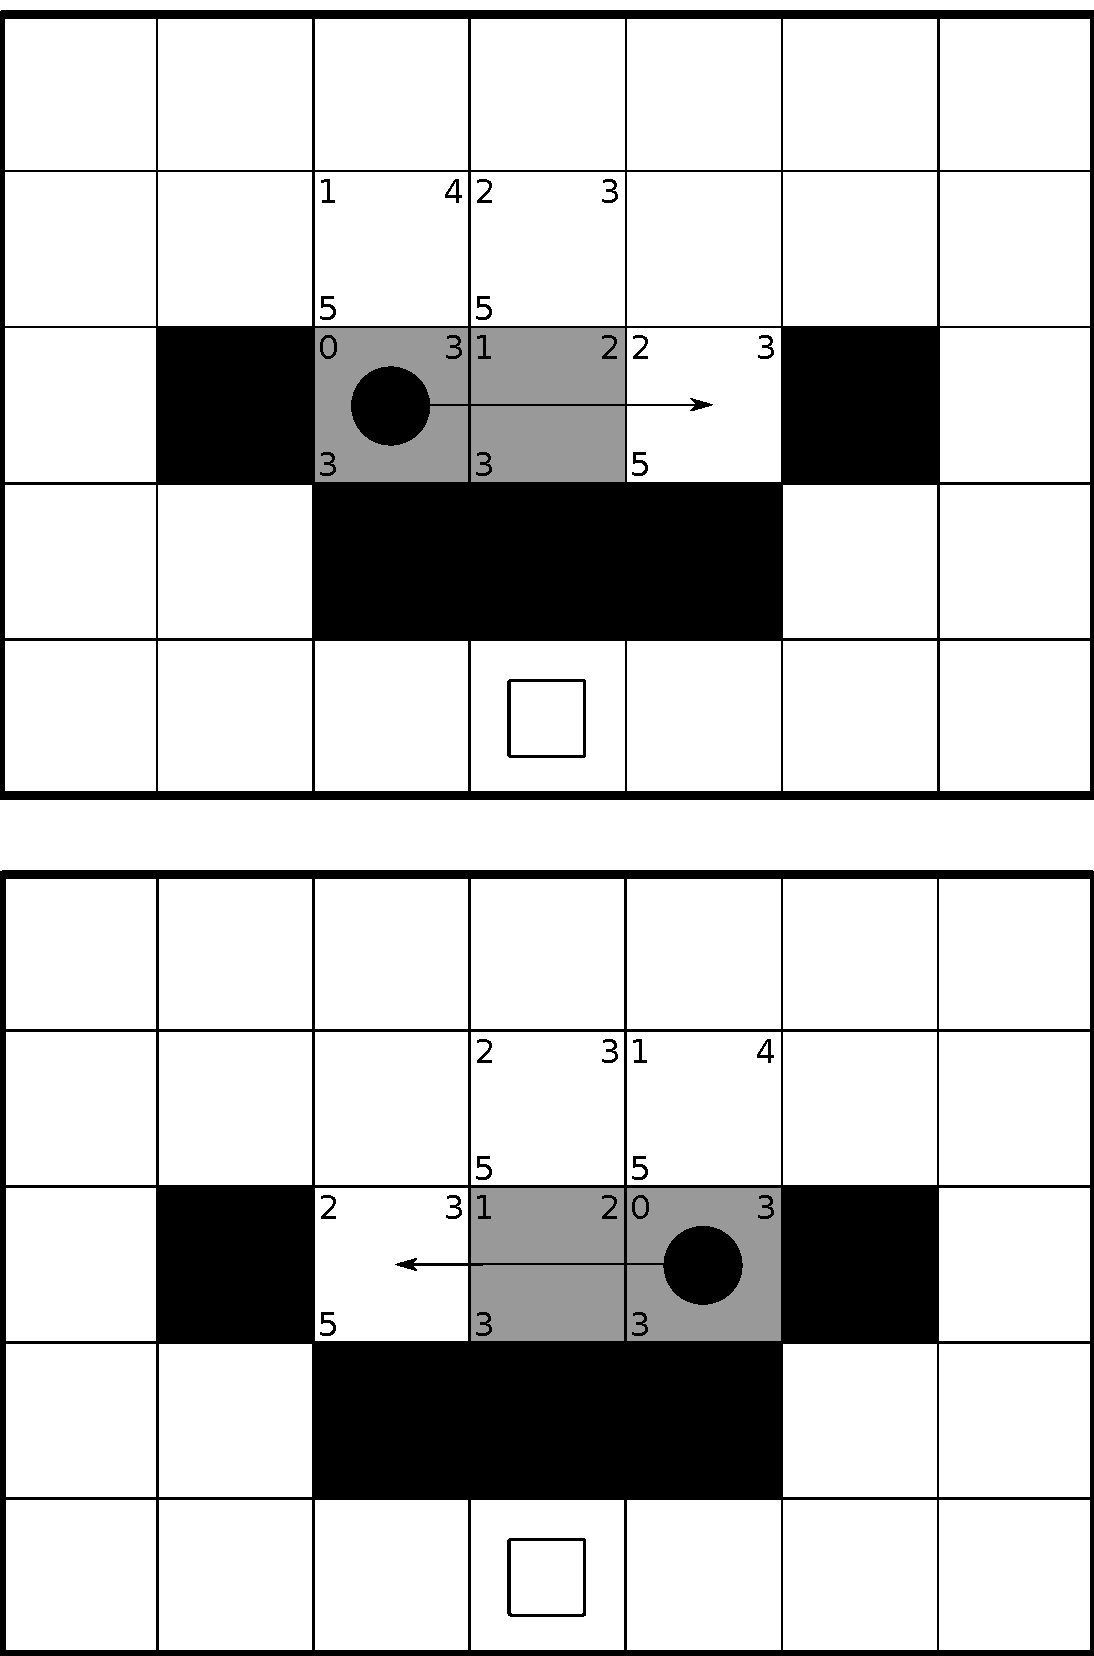
\includegraphics[width=0.45\linewidth]{images/repeatedAStarCycle.pdf}
	\caption{Pojava ciklusa kod ponovljene pretrage}
	\label{fig:pathfindingCycle}
\end{figure} 

\par S obzirom na činjenicu da svaka pretraga kreće ispočetka, moguća je pojava ciklusa. 

\par Na slici~\ref{fig:pathfindingCycle} prikazan je rezultat pretrage koja je rezultirala ciklusom. 
Radi jednostavnosti, u ovom problemu dopušteni su samo pomaci na izravno susjedna polja.
Broj stanja koja se mogu pretražiti ograničen na 2, te je agent zatim otišao prema idućem čvoru u prioritetom redu. 
Ispunjeni krug predstavlja početni položaj u pretrazi, kvadrat ciljni položaj, dok zasivljeno polje predstavlja pregledano stanje. 
U gornjem lijevom kutu zapisan je trošak puta za čvor \(g(n)\), u gornjem desnom kutu vrijednost heuristike \(h(n)\) te u donjem lijevom kutu vrijednost \(f(n) = g(n) + h(n)\).
U slučaju kada se u prioritetni red doda čvor s vrijednosti koja već postoji, prvi u redu je onaj koji je zadnji dodan.

\subsection{Adaptivni A* u stvarnom vremenu}
\par Kako bi se riješio problem pojave ciklusa, potrebno je sačuvati informacije iz prijašnjih pretraga.
Jedan od algoritama koji nudi takvu mogućnost je adaptivni A* u stvarnom vremenu (engl. \textit{Real-Time Adaptive A*}, u nastavu RTAA*).

\par Neka je potrebno izvesti više A* pretraga s konzistentnom heuristikom i istim ciljnim stanjem no s različitim početnim stanjima. Adaptivni algoritam A* će nakon svake pretrage podesiti heurističke vrijednosti posjećenih stanja kako bi buduće pretrage bile obavještenije\cite{article:RTAAStar}.

\par Neka je \(s_{start}\) početno stanje u pretrazi i \(s\) stanje u lokalnom prostoru stanja. Ako je heuristika \(h\) konzistentna vrijedi relacija:
\[\forall s \in S, h(s_{start}) \leq g(s) + h(s).\]
Drugim riječima, put od početne pozicije do cilja kroz stanje \(s\) nikad neće biti veće od stvarne udaljenosti od početnog stanja do cilja.

\par Ako je stanje \(\overline{s}\) prvo stanje u prioritetnom redu kada je lokalna pretraga završila, uvrštavanjem uvjeta konzistentnosti u gore navedenu formulu dobiva se sljedeći izračun:
\[\forall s \in S, f(\overline{s}) \leq g(s) + h(s)\]
\[\forall s \in S, h(s) \geq f(\overline{s}) - g(s).\]

\par Kao posljedicu toga, za svako posjećeno stanje u pretrazi moguće je napraviti korekciju:
\[h(s) = f(\overline{s}) - g(s).\]

% TODO dodati pseudokod

\section{Grupiranje jedinica}\label{sec:grouping}

\chapter{Implementacija jezgrenih funkcionalnosti}\label{ch:implementation}

\chapter{Zaključak}\label{ch:conclusion}
Zaključak.

\bibliography{literatura}
\bibliographystyle{fer}

\begin{sazetak}
Računalne igre jedan su od vrlo značajnih pokretača razvoja računala. Postoji mnoštvo vrsta računalnih igara. 
Jednu od vrlo interesantnih vrsta igara čine strategije u stvarnom vremenu (engl. Real-Time Strategy, RTS). 
Razvoj takvih igara općenito uključuje pisanje mnogih podsustava i razvoj funkcionalnosti koje nisu specifične za konkretnu igru već ih je moguće višestruko iskorištavati. 
Takve funkcionalnosti moguće je izolirati u zaseban razvojni okvir. U okviru završnog rada potrebno je proučiti koji su sve elementi prisutni u RTS igri. 
Potrebno je napraviti programsku implementaciju osnovnih podsustava koje će biti moguće dijeliti između različitih RTS-igara. 
Također je potrebno implementirati prototip jedne konkretne igre koja sadrži osnovne elemente poput prikaza mape svijeta, stvaranja građevina različitih funkcija (proizvodnja, obrana) te jedinica, upravljanje jedinicama (grupiranje, zadavanje ciljeva: dolazak na zadani položaj, pucanje, prikupljanje resursa) i osnovno upravljanje protivničkim jedinicama. 
Implementaciju je potrebno ostvariti u programskom jeziku Java. 
Radu je potrebno priložiti algoritme, izvorne kodove i rezultate uz potrebna objašnjenja i dokumentaciju. 
Citirati korištenu literaturu i navesti dobivenu pomoć.

\kljucnerijeci{Ključne riječi, odvojene zarezima.}
\end{sazetak}

\engtitle{Implementation of RTS game core}
\begin{abstract}
Computer games are a significant catalyst in the development of computers. 
There are many genres of computer games. 
Real-Time Strategy games represent one of the more interesting genres. 
The development of those types of games is based on developing a variety of subsystems and functionalities which aren't specific for one game, and are thus fit for reuse. 
These functionalities can be isolated into a separate workspace. 
As part of thesis, it is necessary to study which elements are present in an RTS game and develop a program implementation of the basic subsystems which can be shared between various RTS games. 
A further requirement is to develop a game prototype which contains the basic elements, such as the construction of buildings with various functions (manufactory, defense) and units, the management of units (grouping, assigning a goal: arrival at a destination, shooting, resource gathering) and basic enemy control.
The implementation is to be written in the Java programming language. 
The completed assignment must be handed over along with the used algorithms, source code and results with the necessary explanations and documentation. 
The literature that was used must be cited along with the received help.

\keywords{Keywords.}
\end{abstract}

\end{document}